\subsection{Scenario II: Uniform Current Drift}
\label{sec:eval:s2}
\begin{figure*}[!t]
\centering
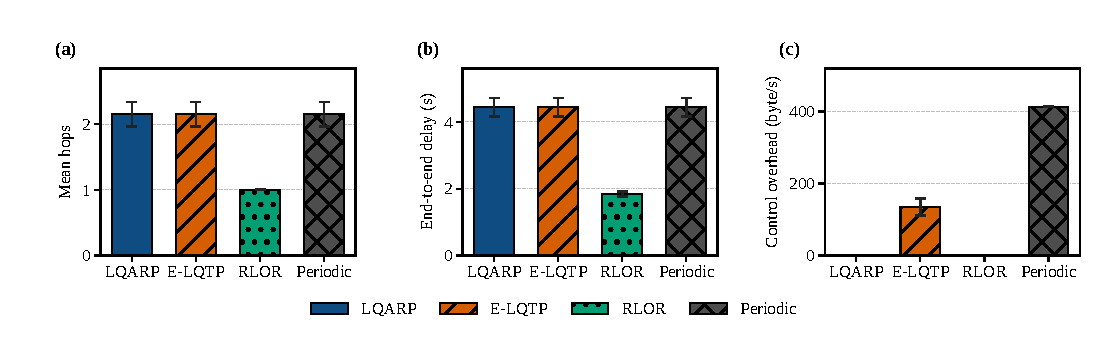
\includegraphics[width=\textwidth]{elqtp_figs/fig3_scenario2_protocols}
\caption{Scenario~II at $2\,\mathrm{m/s}$: hops, delay, and
$O_{\mathrm{ctrl}}$. Error bars are the five-seed sample standard
deviation.}
\label{fig:scenario2_protocols}
\end{figure*}

\begin{figure*}[!t]
\centering
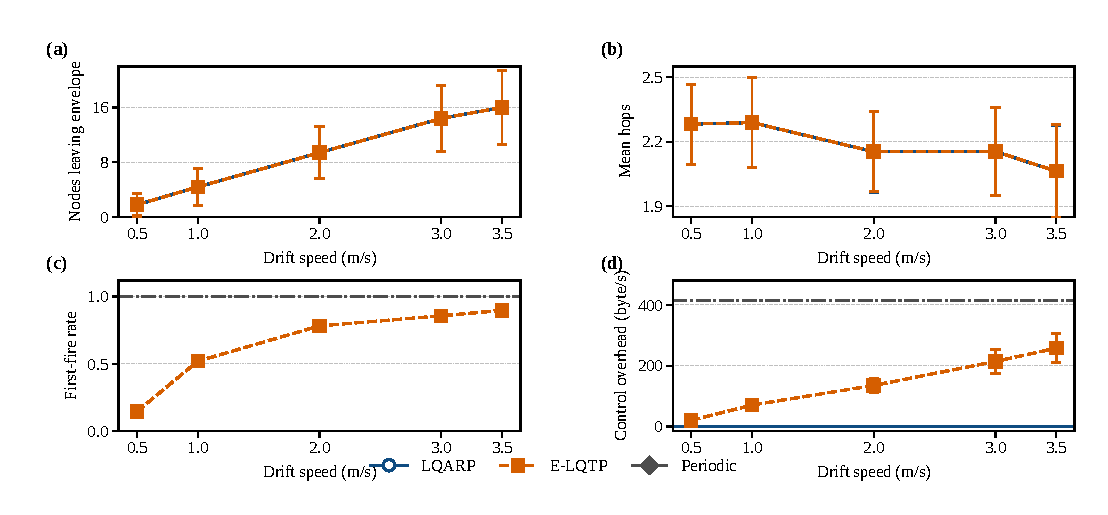
\includegraphics[width=\textwidth]{elqtp_figs/fig4_scenario2_drift}
\caption{Scenario~II versus drift: exits, hops, first-fire, and
$O_{\mathrm{ctrl}}$. Error bars are the five-seed sample standard
deviation.}
\label{fig:scenario2_drift}
\end{figure*}

Table~\ref{tab:s2_protocols} and Fig.~\ref{fig:scenario2_protocols}
compare the four protocols at the reported midpoint
$\|v_{\mathrm{drift}}\|=2\,\mathrm{m/s}$.
E-LQTP reproduces LQARP's data plane---PDR $0.9992\pm 0.0019$,
hops $2.154$ versus $2.153$, delay $4.439\,\mathrm{s}$ versus
$4.438\,\mathrm{s}$, identical $E_{\mathrm{bit}}$ at the printed
precision, identical node-exit packet losses
($0.60\pm 1.34$), VOID $=0$---and cuts control traffic from the
analytic $413.42\,\mathrm{byte/s}$ grid to
$135\pm 23\,\mathrm{byte/s}$ ($0.33\times$, never above $163$).
First-fire is $0.782\pm 0.042$.
By the definition in Section~\ref{sec:eval:metrics} this is the
fraction of live AUV--AUV pairs that record at least one rising
edge.
The true AUV--AUV range rate is zero once both velocities are known.
Those pairs still fire because the velocity hold begins at zero, so
the forecast initially integrates the observer's own drift.
After the hold is written, the constant-velocity model matches the
shared current.
Links to the fixed sink retain a nonzero range rate after that
write.
Fixed-Periodic at $\beta_1=\beta_2=0$ is LQARP's data plane plus
that flat HELLO grid on the shared live pose of
Section~\ref{sec:design:pkt}, which isolates the timer from the
reward.
RLOR-inspired again sits at one hop ($T_{\mathrm{e2e}}=1.845\,\mathrm{s}$)
because the sink remains in $N_{\mathrm{SNR}}$ for live relays; it
has no dedicated control plane.

% Scenario II four-protocol headline. Wide 7-col: stay table*.

\begin{table*}[!t]
\caption{Scenario~II at $2\,\mathrm{m/s}$ ($N=40$, five seeds,
$\beta_1=\beta_2=0$). Entries with $\pm$ are the sample standard
deviation. VOID $=0$.}
\label{tab:s2_protocols}
\centering
\small
\begin{tabular}{lcccccc}
\hline
Protocol & PDR & $T_{\mathrm{e2e}}$ (s) & $E_{\mathrm{bit}}$
  & $O_{\mathrm{ctrl}}$ & Hops & First-fire \\
\hline
LQARP & $0.9992\pm 0.0019$ & $4.438\pm 0.277$ & $1.156\pm 0.100\times 10^{-2}$
  & $0$ & $2.153\pm 0.187$ & --- \\
E-LQTP & $0.9992\pm 0.0019$ & $4.439\pm 0.277$ & $1.156\pm 0.100\times 10^{-2}$
  & $135\pm 23$ & $2.154\pm 0.187$ & $0.782\pm 0.042$ \\
RLOR-insp. & $1.0000\pm 0$ & $1.845\pm 0.074$ & $5.362\times 10^{-3}$
  & $0$ & $1.000\pm 0.001$ & --- \\
Periodic & $0.9992\pm 0.0019$ & $4.438\pm 0.277$ & $1.156\pm 0.100\times 10^{-2}$
  & $413.42$ & $2.153\pm 0.187$ & $1.000$ \\
\hline
\end{tabular}
\end{table*}


Table~\ref{tab:s2_drift} and Fig.~\ref{fig:scenario2_drift} sweep
drift magnitude.
The hop ratio E-LQTP/LQARP is $1.000\times$ at every $v$.
PDR, delay, and node-exit packet losses match LQARP at every $v$.
Energy per data bit agrees with LQARP through the digits of
Table~\ref{tab:s2_protocols}; across the sweep the largest
relative difference is below $3\times 10^{-4}$.
$O_{\mathrm{ctrl}}$ over the periodic $413.4\,\mathrm{byte/s}$ is
$0.05\times$, $0.17\times$, $0.33\times$, $0.52\times$, and
$0.62\times$ at $0.5$, $1$, $2$, $3$, and $3.5\,\mathrm{m/s}$.
First-fire rises with drift, $15\%\to 52\%\to 78\%\to 86\%\to 90\%$.
Panel~(a) of Fig.~\ref{fig:scenario2_drift} is envelope exits, not
PDR: the two protocols lose the same relays.
Even at $3.5\,\mathrm{m/s}$ E-LQTP stays under the periodic budget.

% Scenario II drift sweep. Wide 7-col: stay table*.

\begin{table*}[!t]
\caption{Scenario~II versus drift (LQARP vs.\ E-LQTP; five seeds,
$\beta_1=\beta_2=0$). Hop ratio $1.000\times$ at every $v$.}
\label{tab:s2_drift}
\centering
\small
\begin{tabular}{ccccccc}
\hline
$v$ (m/s) & Protocol & PDR & $T_{\mathrm{e2e}}$ (s) & $O_{\mathrm{ctrl}}$
  & Hops & First-fire \\
\hline
$0.5$ & LQARP & $1.000$ & $4.776\pm 0.403$ & $0$ & $2.282\pm 0.186$ & --- \\
$0.5$ & E-LQTP & $1.000$ & $4.776\pm 0.403$ & $20.2\pm 4.2$ & $2.282\pm 0.186$ & $0.146\pm 0.021$ \\
$1.0$ & LQARP & $0.9995\pm 0.0012$ & $4.752\pm 0.377$ & $0$ & $2.289\pm 0.208$ & --- \\
$1.0$ & E-LQTP & $0.9995\pm 0.0012$ & $4.752\pm 0.377$ & $70.7\pm 6.2$ & $2.289\pm 0.208$ & $0.520\pm 0.031$ \\
$2.0$ & LQARP & $0.9992\pm 0.0019$ & $4.438\pm 0.277$ & $0$ & $2.153\pm 0.187$ & --- \\
$2.0$ & E-LQTP & $0.9992\pm 0.0019$ & $4.439\pm 0.277$ & $135.1\pm 23.1$ & $2.154\pm 0.187$ & $0.782\pm 0.042$ \\
$3.0$ & LQARP & $1.000$ & $4.431\pm 0.333$ & $0$ & $2.154\pm 0.203$ & --- \\
$3.0$ & E-LQTP & $1.000$ & $4.433\pm 0.331$ & $213.8\pm 39.1$ & $2.155\pm 0.203$ & $0.857\pm 0.034$ \\
$3.5$ & LQARP & $1.000$ & $4.200\pm 0.393$ & $0$ & $2.063\pm 0.215$ & --- \\
$3.5$ & E-LQTP & $1.000$ & $4.200\pm 0.393$ & $257.7\pm 46.9$ & $2.063\pm 0.215$ & $0.897\pm 0.028$ \\
\hline
\end{tabular}
\end{table*}

